\documentclass[onecolumn,11pt]{article}
%*********
%Paquetes
%*********
\usepackage[english]{babel}
\usepackage[utf8]{inputenc}
\usepackage[a4paper, total={7in, 9in}]{geometry}
\usepackage{amsfonts}
\usepackage{dsfont}
\usepackage{physics}
\usepackage[dvipsnames]{xcolor}
\usepackage{tikz-cd} %para diagrama conmutatitvo
\usepackage{multicol} 
\usepackage{hyperref}
\usepackage{caption}
\usepackage{subcaption}
\usepackage{wrapfig}
\usepackage{tcolorbox}
\usepackage{setspace}
\setstretch{1.2}
\listfiles

%*********
%Comandos
%*********
% Default fixed font does not support bold face
\DeclareFixedFont{\ttb}{T1}{txtt}{bx}{n}{9} % for bold
\DeclareFixedFont{\ttm}{T1}{txtt}{m}{n}{9}  % for normal

% Custom colors
\usepackage{color}
\definecolor{deepblue}{rgb}{0,0,0.5}
\definecolor{deepred}{rgb}{0.6,0,0}
\definecolor{deepgreen}{rgb}{0,0.5,0}

\usepackage{listings}

% Python style for highlighting
\newcommand\pythonstyle{\lstset{
language=Python,
basicstyle=\ttm,
morekeywords={self},              % Add keywords here
keywordstyle=\ttb\color{deepblue},
emph={MyClass,__init__},          % Custom highlighting
emphstyle=\ttb\color{deepred},    % Custom highlighting style
stringstyle=\color{deepgreen},
frame=tb,                         % Any extra options here
showstringspaces=false
}}

% Python environment
\lstnewenvironment{python}[1][]
{
\pythonstyle
\lstset{#1}
}
{}

% Python for external files
\newcommand\pythonexternal[2][]{{
\pythonstyle
\lstinputlisting[#1]{#2}}}

% Python for inline
\newcommand\pythoninline[1]{{\pythonstyle\lstinline!#1!}}



\title{Stage au IPCMS}
\author{Autores}
\date{}

\begin{document}
\maketitle
\tableofcontents
\newpage
\section*{Gossaire}

\textbf{résonance ferromagnétique} : C'est le couplage entre une onde éléctromagnetique et la aimantation du matériau à travers lequel elle passe. L'onde perd de l'énergie qui est absorbée par la précession de Larmor du matériau\\
\textbf{exchange bias}\\
\textbf{magnetocrystalline anisotropy}
\newpage
\section{Semaine 1}

J'ai rien écrit pour cette semaine. Cependant, j'ai décidé d'utiliser cette section pour écrire plusieurs concepts de théorie dont j'aurai besoin.

\subsection{Théorie des antennes}

\subsection{Magnons antiferromagnetiques}

\subsection{Améliorer émission THz avec antennes plannes}
\newpage
\section{Semaine 2 - 12 fev}

\subsection{Lundi}

Lundi on a travaillé sur le logiciel CST. On a modelisé un antenne
dipolaire en or avec un substrat en Silicium sans pertes. L'idée
était un peu de jouer et de se familiariser avec le logiciel.

De ma part, j'ai varié le gap enter les deux brins pour obtenir le facteur S
en fonction de la fréquence pour plusieurs valeurs du gap. Cependant, j'ai oublié
de changer aussi la taille des brins. Cela veut dire qu'à chaque fois que je changeais
le gap, la taille totale de l'antenne changeait aussi. Or, il fallair changer le gap
en gardant la taille totale de l'antenne constante. J'ai pas eu le temps de corriger 
cette erreur.

\subsection{Mardi}

Mardi on a travaillé sur le problème de l'enveloppe des signaux qu'on a obtenu la
seaine dernière. Victor a fait un code qui trouve les valeurs maximales en utilisant
\textsc{np.argmax}. Moi j'ai trouvé un code sur Stackexchange qui le fait en calculant
un changement de signe sur la dérivée du signal. 

Après il a commencé à travailler sur les antennes de papillon. Moi j'ai organisé tout et 
j'ai créé un github.
\newpage
\section{Semaine 3 - 19 fev}

\subsection{Lundi}

Normalement on allait obtenir l'optimization pour les antennes, mais on n'arrive même pas à
réproduire les résultats de Matthias Pacé. Demain on va continuer.

\subsection{Mardi}

On n'arrive pas a trouver les mêmes résultats que Matthias. Parce qu'on n'arrive pas avec le bowtie, on a
decidé d'essayer d'abord avec l'antenne dipolaire. Je ne suis pas arrivé à le faire. C'est Mathieu qui a 
trouvé la solution, montrée sur la Figure \ref{fig:first_dipole}. En fait il fallait construire le port à 
travers le mode \textit{pick edge}. Je ne suis pas sûr de pourquoi ca change tellement.
J'ai dans mes notes une formule pour calculer l'impendance du port, et je suis arrivé a obtenir l'impendance
correcte pour l'antenne de bowtie, mais je ne comprends pas la formule.

\begin{figure}[h!]
    \centering
    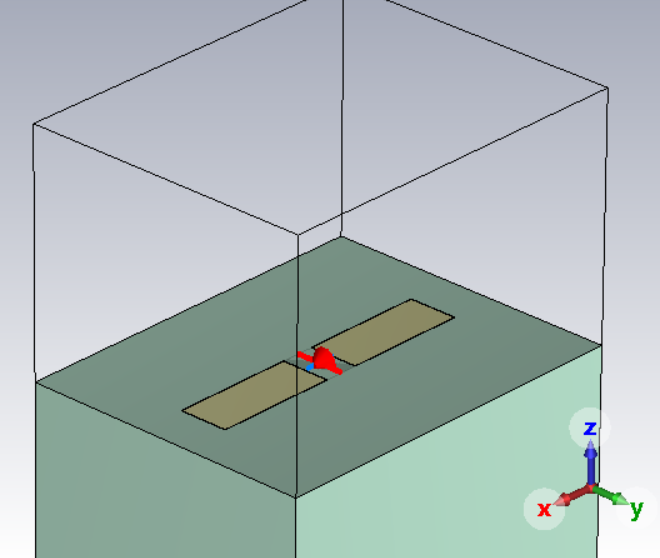
\includegraphics[width=0.35\textwidth]{texfigures/first_dipole.png}
    \caption{\label{fig:first_dipole} Une antenne dipolaire en or sur un substrat de saphire (Alumina au $96\%$ sans pertes). Les dimensions sont $57\mu$m pour la longueur totale de l'antenne, $7\mu$m pour le gap, $10\mu$m pour la base de l'antenne, et $0.1\mu$m pour l'épaisseur.}
\end{figure}


Victor a codé pendant toute la journée. On a aussi commencé à travailler avec GitHub. On a aussi assisté
à un séminaire sur des modèles théoriques pour la création de nouveaux pigments. C'était intéressant.
\newpage
\section{Semaine 4 - 26 fev}

\subsection{Lundi}

L'\textbf{objectif} d'aujourd'hui c'est de
\begin{itemize}
    \item Optimiser la bowtie simple
    \item Optimiser la bowtie vraie
    \item Optimiser la dipole
\end{itemize}

Pour les simulations, on a maintenant ajouté une couche d'oxide SiO$_{2}$. C'est cela qu'on voit dans la figure \ref{fig:oxide_film}.

\begin{wrapfigure}{R}{0.4\textwidth}
    \centering
    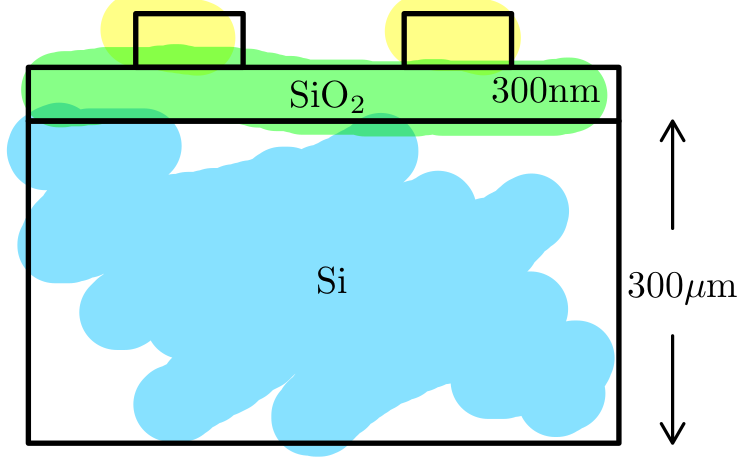
\includegraphics[width=0.35\textwidth]{texfigures/ocide_film.png}
    \caption{\label{fig:oxide_film} On ajoute une couche d'oxide au dessus du substrat.}
\end{wrapfigure}
\newpage
\section{Semaine 5 - 11 mars}
\newpage
\section{Semaine 6 - 18 mars}

Cette semaine je n'ai pas été au IPCMS. Victor a travaillé.

\newpage
\section{Semaine 7 - 25 mars}

\subsection{Lundi}

Aujord'hui j'ai travaillé sur le code de Victor. En gros il a essayé de faire une fonction 

\section{``In-text'' listing highlighting}

\begin{python}
class MyClass(Yourclass):
    def __init__(self, my, yours):
        bla = '5 1 2 3 4'
        print bla
\end{python}

\section{External listing highlighting}

%\pythonexternal{}

\section{Inline highlighting}

Definition \pythoninline{class MyClass} means \dots

\subsection{Mardi}


\newpage
\end{document}
